\documentclass[11pt, oneside]{article}   	% use "amsart" instead of "article" for AMSLaTeX format
\usepackage{geometry}                		% See geometry.pdf to learn the layout options. There are lots.
\geometry{letterpaper}                   		% ... or a4paper or a5paper or ... 
%\geometry{landscape}                		% Activate for for rotated page geometry
%\usepackage[parfill]{parskip}    		% Activate to begin paragraphs with an empty line rather than an indent
\usepackage{graphicx}				% Use pdf, png, jpg, or eps� with pdflatex; use eps in DVI mode
								% TeX will automatically convert eps --> pdf in pdflatex		
\usepackage{amssymb}
\usepackage{amsmath}
\usepackage{algorithm2e}

\usepackage{ifthen,version}
\usepackage[usenames,dvipsnames]{color}
\newboolean{include-notes}
\setboolean{include-notes}{true}
\DeclareRobustCommand{\jknote}[1]{\ifthenelse{\boolean{include-notes}}%
	{\textcolor{Maroon}{\textbf{JK: #1}}}{}}

\title{Notes on Reconfiguration Among Clutter}
%\date{}							% Activate to display a given date or no date

\begin{document}
\maketitle

\section*{Introduction}
In these notes we examine the problem of grasping an object in a cluttered environment.  We categorize the clutter into two groups: static and movable objects. We allow the robot to push any movable object in order to clear a path for grasping the target object.  The robot must avoid contact with static obstacles.  

\section*{Related Work}


\section*{Problem Formulation}
We now provide a more formal description of the problem and introduce notation used throughout the remainder of these notes. As stated previously, we wish to solve the problem of grasping an object, $G$, in a cluttered environment.  Specifically, we say that we have a robot operating in an environment with both static and movable objects.  Let $O = \{O_1, ..., O_k\}$ be the set of static objects.  These objects should be treated as obstacles. Contact between the robot and these objects is forbidden.  Let $M = \{M_1,...,M_n\}$ be a set of movable objects.  These objects can be displaced via contact with the robot. We require that this displacement does not introduce contact between any two objects in $M$ nor does it introduce contact between an object in $M$ and an object in $O$.  Finally, we cannot introduce contact between any object in $M$ and our goal object $G$.  We treat our goal object as a movable object and identify the same contact constraints as any object in $M$, but identify it separately.  We say that a movable object can be displaced when the robot is touching the object.

Let $C_R$ identify the configuration space of the robot.  Let $G_R$ identify the configuration space of the target object, $G$. We can define our goal as a set of configurations, $Q_G = \{q_t \in C_R | f(q_t, g_t) = 0 \}$, where $f(q_t, g_t) = 0$ when our goal object in pose $g_t$ can be stably grasped by the robot in configuration $q_t$.  Let $C_{M_i}$ represent the configuration space of $M_i$.  We can then formalize our problem as follows: given an initial configuration of the robot, $q_0 \in C_R$, an initial configuration of the target object, $g_0 \in G_R$ and an initial configuration for each movable objects, $(c^{M_1}_0,...,c^{M_n}_0) \in (C_{M_1},...,C_{M_n})$, we want to find a path from $q_0$ to any configuration $q_t \in Q_G$ that is collision-free.  

\subsection*{Events}
\jknote{I think this section is irrelevant. But I will leave it for now.}
Here we define the concept of a "contact event."  We define a set of contact indicators, $(I^{M_1},...,I^{M_n}) \in \{0,1\}$ where $I^{M_i} = 1$ if the robot is in contact with movable object $M_i$ and $0$ otherwise.  We can then say a contact event is one where $I^{M_i}_{t-1} \neq I^{M_i}_{t}$ for any $i$.  Informally, we define such an event as any moment in which the contact state between the robot and a movable object changes.  

\subsection*{Actions}
Ultimately we wish to produce a path defined by a sequence of actions, $a_0,...,a_m$ such that when applied to the end-effector starting at pose $q_0$ the resulting state is a state with end-effector at pose $q_m \in Q_G$.  We can parameterize these actions as follows:
\[a_t = \left[ \dot{v}, \dot{\theta}, \dot{a}, \Delta t \right] \]
where $\dot{v}$ is the forward velocity of the manipulator, $\dot{\theta}$ is the rotational velocity of the manipulator, $\dot{a}$ is the aperture of the end-effector and $\Delta t$ is the maximum duration of the action.

\begin{figure}[htbp]
\begin{center}
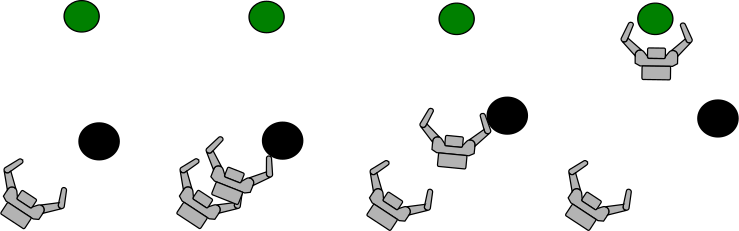
\includegraphics[width=0.8\textwidth]{action_events}
\caption{Forward simulation of an action. (a) The end-effector starts free of contact with any objects. (b) During execution, contact is made with movable object (black disc). (c) The movable object is pushed out of the way. (d) The end-effector continues on to achieve a valid grasp configuration.}
\label{fig:action_events}
\end{center}
\end{figure}
We note that an action can encompass multiple events.  Consider the action depicted in Figure~\ref{fig:action_events}.  During execution of this action, the robot starts out of contact with any movable obstacle(Figure~\ref{fig:action_events}(a)).  The robot then makes contact with a movable obstacle, triggering a contact event (Figure~\ref{fig:action_events}(b)).  After pushing the obstacle out of the way the robot loses contact with the obstacle, triggering a second contact event (Figure~\ref{fig:action_events}(c)).  Thus we can say we have a one-to-many relationship between actions and events.  

We define two action classes.  \textit{transit} and \textit{transfer}.  \textit{Transit} actions are those with zero contact events occurring.  In other words, they represent actions where the end-effector moves without pushing any movable objects.  \textit{Transfer} actions are those with one or more contact events.  These represents actions where one or more movable objects are pushed during execution of the action.

\section*{Forward Search}
\begin{algorithm}
\SetKwFunction{ContainsGoal}{ContainsGoal}
\SetKwFunction{Different}{Different}
\SetKwFunction{InitTree}{InitTree}
\SetKwFunction{Sample}{SampleConfiguration}
\SetKwFunction{Nearest}{NearestNeighbor}
\SetKwFunction{Extend}{Extend}
\KwIn{ the start node $s_{0}$ }
\KwOut{ the tree $T$ }
\BlankLine
$T \leftarrow$ \InitTree($s_{0}$) \;
\While{not \ContainsGoal{$T$}} {
$s_{rand} \gets$ \Sample{} \;
$s_{near} \gets$ \Nearest{$T$, $s_{rand}$} \;
$s_{new} \gets$ \Extend{$T$, $s_{near}$, $s_{rand}$} \;
\If{\Different{$s_{new}$, $s_{near}$}} {
$T$.add\_vertex($s_{new}$) \;
$T$.add\_edge($s_{near}$, $s_{new}$) \;
}
}
\label{alg:rrt}
\caption{The basic RRT algorithm}
\end{algorithm}
We can utilize an RRT to perform a forward search through our space starting from the initial state of the environment $s_0$ where:
\[s_0 =\left[q_0, g_0, c^{M_1}_0,...,c^{M_n}_0\right]\]
The RRT algorithm can be seen in Algorithm~\ref{alg:rrt}.  We detail specifics of the important functions in the algorithm now.

\subsection*{SampleConfiguration}
\begin{figure}[htbp]
\begin{center}
\includegraphics[width=0.8\textwidth]{object_projection}
\end{center}
\caption{A sample project of an object initially sampled in collision with the end-effector.}
\label{fig:object_projection}
\end{figure}
The SampleConfiguration function samples a state, $s_{rand}$, in the following manor:
\begin{enumerate}
\item Sample a collision free $q_{rand}$ from the configuration space of the end-effector, $C_R$.  In this step, only collisions with the static objects, $\{O_1,...O_k\}$, are considered.
\item Let $g_{rand}=g_0$.  If $g_{rand}$ is in collision with $q_{rand}$, apply a projection which moves $g_{rand}$ so that it is touching the closest point on the end-effector. Figure~\ref{fig:object_projection} shows a sample projection.
\item Sample poses for each object $O^j_{rand} = O^j_0$.  Similar to the goal, if the sample generates a collision between the end-effector pose, $q_{rand}$, the goal pose $g_{rand}$ or any already sampled object poses, $\{O^1_{rand},...,O^{j-1}_{rand}\}$, apply a projection to move the object out of collision.
\end{enumerate}
\jknote{Is all this a)correct and b)necessary? In the Simeon paper they actually just set the movable objects and goal to their respective start poses, then sample a free $q_{rand}$ treating the goal and the movable objects as static and ensuring the sampled $q_{rand}$ isn't in collision.}

\subsection*{NearestNeighbor}
To define the NearestNeighbor function we need to implement a distance metric.  For our metric we choose the norm of the distance between the two state vectors:
\[ d(s_j, s_k) = \left| s_j - s_k\right| \]

\subsection*{Extend} 
\label{sec:extend}

During execution of the Extend function, we forward simulate each action starting with the environment in state $s_{near}$ until one of the following stop criteria is encountered:
\begin{enumerate}
\item The simulation time has exceeded the maximum duration, $\Delta t$, defined for the action.
\item The simulation has produced a collision with an obstacle in the environment.
\item The simulation has produced a collision between a movable object and an obstacle.
\item The simulation has produced a collision between two movable objects.
\end{enumerate}
Once the action is stopped, $s'_{near}$ will be generated based on the state at that instance in the simulation.  Formally, we say that we have a one-to-one mapping $T$ between start-state/action pairs and end-state:
\[ s'_{near} = T(s_{near}, a) \]
Then Extend function searches for the action, $a_t$, which produces the $s'_{near}$ closest to the randomly sampled $s_{rand}$. Formally:
\[ a_t = \arg\min_{a \in A} d\left(s_{rand}, T(s_{near}, a)\right) \]
During forward simulation, any contact between the robot and a movable object will trigger the robot to push the object.  We assume quasi-static interactions between the robot and the pushed object.  
\jknote{Maybe add in here a brief section describing quasi-static physics}

\section*{Backward Search}
\begin{figure}[htbp]
\begin{center}
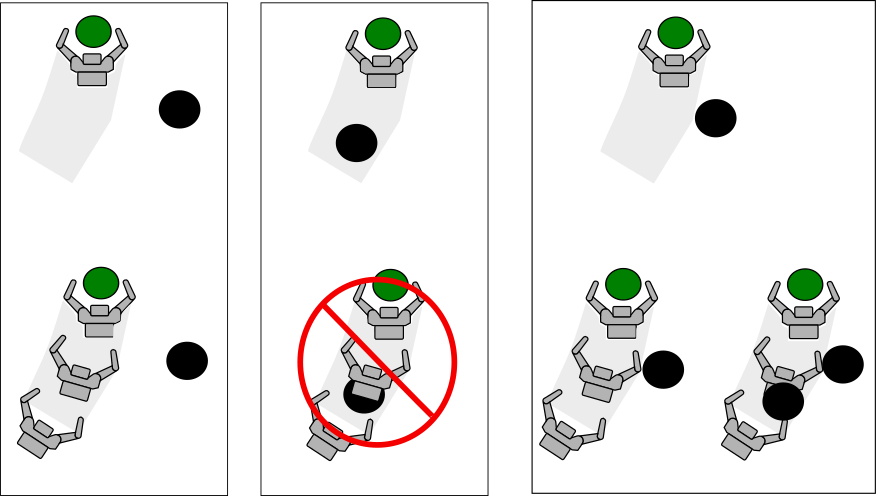
\includegraphics[width=0.8\textwidth]{backwards_search}
\caption{Three possible scenarios encountered during backward search.  In each of the three images, the top picture represents the state we are performing the backwards search from.  The black disc represents a movable object.  The green disc represents the goal.  The gray region represents the swept volume of the end-effector during action execution. (a) The swept volume of the end-effector makes no contact with the swept volume.  Here there is a single state that represents the configuration of the world at the start of the action. (b) A movable object is in the swept volume.  Here there is no possible previous world state, as the motion of the end-effector would have moved that object during action execution. (c) Here an object is touching the edge of the footprint of the end-effector.  In this case there are infinite states that represent the world at the start of the action.  Shown are two.  The first represents a object not being pushed. but instead starting in a pose on the edge of the swept volume.  The second represents the object starting in contact with the manipulator and being pushed out of the way. }
\label{fig:backwards_search}
\end{center}
\end{figure}
\begin{algorithm}
\SetKwFunction{ContainsGoal}{ContainsGoal}
\SetKwFunction{Different}{Different}
\SetKwFunction{InitTree}{InitTree}
\SetKwFunction{Sample}{SampleConfiguration}
\SetKwFunction{Nearest}{NearestNeighbor}
\SetKwFunction{Extend}{Extend}
\SetKwFunction{Running}{Running}
\SetKwFunction{AddGoal}{AddGoal}
\SetKwFunction{ExtractPath}{ExtractPath}
\SetKwFunction{Swap}{Swap}
\KwIn{ the start node $s_{0}$ }
\KwIn{ $p_{sample}$ }
\KwOut{ the tree $T$ }
\BlankLine
$T_{start} \leftarrow$ \InitTree($s_{0}$) \;
$T_{goal} \leftarrow$ \InitTree(NULL) \;
$T_a \gets T_{start}$ \;
$T_b \gets T_{goal}$ \;
\While{ \Running{} } {
\If{$T_{goal}.size = 0$ or $rand(0,1) < p_{sample}$}{
\AddGoal($T_{goal}$)
}
{
$s_{rand} \gets$ \Sample{} \;
$s_{near}^a \gets$ \Nearest{$T_a$, $s_{rand}$} \;
$s_{reached}^a \gets$ \Extend{$T_a$, $s_{near}^a$, $s_{rand}$} \;
$T_a$.add\_vertex($s_{reached}^a$) \;
$T_a$.add\_edge($s_{near}^a$, $s_{reached}^a$) \;
$s_{near}^b \gets$ \Nearest($T_b$, $s_{reached}^a$) \;
$s_{reached}^b \gets$ \Extend($T_b$, $s_{near}^b$, $s_{reached}^a$) \;
$T_b$.add\_vertex($s_{reached}^b$) \;
$T_b$.add\_edge($s_{near}^b$, $s_{reached}^b$) \;
\If{$s_{reached}^a = s_{reached}^b$} {
$P \gets$ \ExtractPath($T_a$, $s_{reached}^a$, $T_b$, $s_{reached}^b$) \;
return $P$
}{
\Swap($T_a$, $T_b$) \;
}}}
\label{alg:gsrrtconnect}
\caption{The RRT-Connect algorithm with Goal Sets}
\end{algorithm}
While forward search will allow for generating feasible plans for grasping the object, we wish to speed planning via use of the RRT-Connect planner, which maintains two trees, one grown from the start and one from the goal, and attempts to connect them(Algorithm~\ref{alg:gsrrtconnect}).  We note that we use the Goal Set modification to the RRT-Connect algorithm to account for our underspecified goal.

In order to build a tree grown backwards from the goal, we need a method for backwards simulating a pushing action.  Introducing this backwards simulation poses challenges not present in the forward search.  Figure~\ref{fig:backwards_search} shows the three situations that can be encountered. In the left most figure, backwards simulation of the action shows no intersection between the footprint of the end-effector and the movable object (black circle).  Thus there is a one-to-one mapping between the end-state and the start-state.  In the middle figure, a movable object sits in the footprint of the action.  This renders the action impossible, as there is no way the end-effector could have swept that volume of space without moving the object or having a collision which stopped the action earlier.  The figure on the right shows the most interesting case.  Here there is a movable object that is touching the edge of the swept volume of the end-effector.  This case introduces a one-to-many mapping between the start state and this end state.  Two such mappings are shown in the figure.  The first shows a scene where the object was not pushed during the action, but instead just happened to be sitting on the edge of the action space.  The second shows the object in the swept volume at the start of the action. During execution of the action the object is pushed to the final resting location.  In this case there are an infinite number of possible states that could have started the action.  Each of these states differ only in where the object started, or equivalently where the push would start during action execution.

\begin{figure}[htbp]
\begin{center}
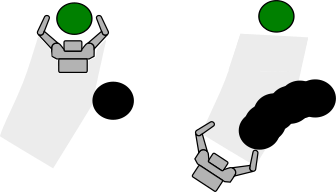
\includegraphics[width=0.5\textwidth]{pre_image}
\caption{The results of backwards simulation of a single action from a goal state.  The bottom left figure represents a pure transit, where the moveable object (black disc) is not pushed by the end-effector.  The bottom right figure represents the transfer action.  In this action, the movable object was pushed by the manipulator to its final resting location.  Here the black region represents the set of pre-image of the movable object (the set of all possible start locations).}
\label{fig:pre_image}
\end{center}
\end{figure}
In order to enable the use of a bi-directional search strategy, we must decide on a method for handling this ambiguity in the reverse search.  For this we will define the notion of pre-image \jknote{Need a better word. Pretty sure the notion of pre-image is well defined in a different way}.  We say the pre-image of an object is the set of all configurations that an object could have started in such that it ended in its final location.  Formally, we define:
\[P^{M_j}_t = \{O^{M_j}_t \in C^{M_j} | T(O^{M_j}_t, a) = O^{M_j}_{t+1} \} \]
We note that in this case we use the mapping $T$ to apply $a$ to a single object rather than an entire state, as was done previously in Section~\ref{sec:extend}.

Figure~\ref{fig:pre_image} shows an example pre-image for an object being pushed.  The pre-image represents every pose for the object from which the push could have started. We then modify our state to represent the pose of a movable object by its pre-image:
\[s_t =  \left[q_t, g_t, P^{M_1}_t, ...., P^{M_n}_t\right] \]
For the two unambiguous cases in the reverse search (Figure~\ref{fig:backwards_search}(a)(b)), the pre-image will represent a single pose.  In other words, for those cases: $P^{M_j}_t = c^{M_j}_t$.

Using this representation, we can now reduce our infinite number of start locations down to two: the first represents a pure transit by the end-effector, where the object is not pushed.  The second represents the infinite set of transfers. 

Our new state representation requires an adjustment to the distance metric. In particular, we define the distance between two pre-images as follows:
\[ d'(P^{M_i}_j, P^{M_i}_k) = \min_{O^{M_i}_j \in P^{M_i}_j, O^{M_i}_k \in P^{M_i}_k} \left| O^{M_i}_j - O^{M_i}_k \right|^2 \]
Then:
\[ d(s_j, s_k) = \sqrt{\left| q_j - q_k \right|^2 + \left| g_j + g_k \right|^2 + \sum_i d'(P^{M_i}_j, P^{M_i}_k)} \]
\begin{figure}[htbp]
\begin{center}
\includegraphics[width=1.0\textwidth]{example_expansion}
\caption{Pictured is the bi-directional search for an example scenario.  The top left set of states represents the forward search tree rooted at the start state.  The bottom right set of states represent the backward search tree, rooted in a particular goal configuration.  The two states captured in the green box in the middle of the figure indicate where the two trees meet.  These states evaluate as equivalent, allowing for a path through the tree to be found.}
\label{fig:example_expansion}
\end{center}
\end{figure}
\begin{figure}[htbp]
\begin{center}
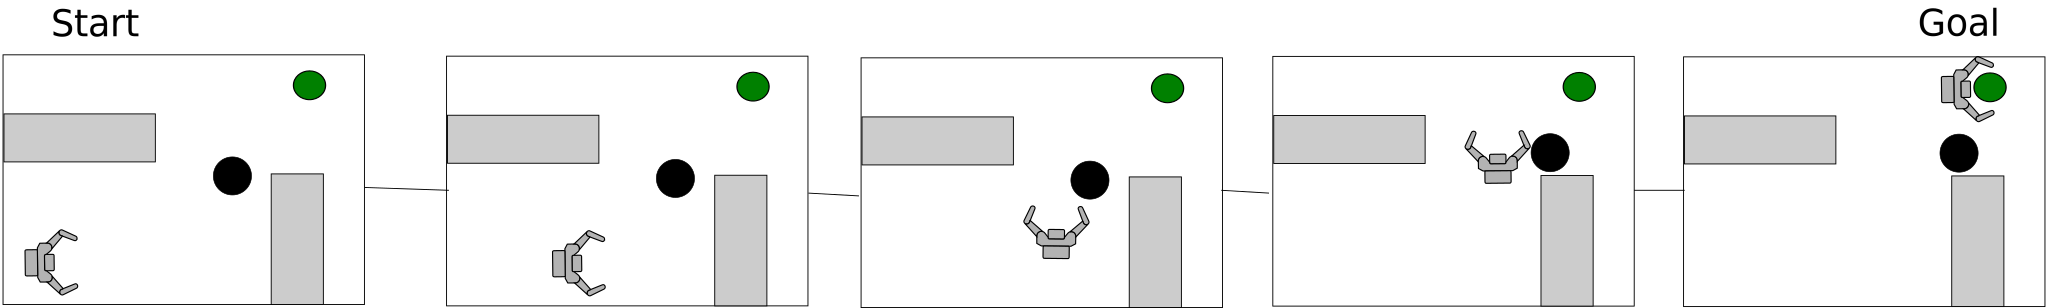
\includegraphics[width=1.0\textwidth]{example_solution}
\caption{The path resulting from the search through the tree built in Figure~\ref{fig:example_expansion}.}
\label{fig:example_solution}
\end{center}
\end{figure}
Figure~\ref{fig:example_expansion} shows growth of the bi-directional search tree for a simple problem.  The two states in the green box in the center of the figure represent equivalent states.  Thus the trees meet when these two states are added to their appropriate subtrees. Figure~\ref{fig:example_solution} represents the final path generated by the search.

\end{document}
